%%%%%%%%%%%%%%%%%%%%%%%%%%%%%%%%%%%%%%%%%
% FRI Data Science_report LaTeX Template
% Version 1.0 (28/1/2020)
% 
% Jure Demšar (jure.demsar@fri.uni-lj.si)
%
% Based on MicromouseSymp article template by:
% Mathias Legrand (legrand.mathias@gmail.com) 
% With extensive modifications by:
% Antonio Valente (antonio.luis.valente@gmail.com)
%
% License:
% CC BY-NC-SA 3.0 (http://creativecommons.org/licenses/by-nc-sa/3.0/)
%
%%%%%%%%%%%%%%%%%%%%%%%%%%%%%%%%%%%%%%%%%


%----------------------------------------------------------------------------------------
%	PACKAGES AND OTHER DOCUMENT CONFIGURATIONS
%----------------------------------------------------------------------------------------
\documentclass[fleqn,moreauthors,10pt]{ds_report}
\usepackage[english]{babel}

\graphicspath{{fig/}}




%----------------------------------------------------------------------------------------
%	ARTICLE INFORMATION
%----------------------------------------------------------------------------------------

% Header
\JournalInfo{FRI Data Science Project Competition 2020}

% Interim or final report
\Archive{Interim report} 
%\Archive{Final report} 

% Article title
\PaperTitle{How good is my plot?} 

% Authors (student competitors) and their info
\Authors{Maruša Oražem, Urša Zrimšek, Andrej Hafner}

% Advisors
\affiliation{\textit{Advisors: Assoc. Prof. dr. Erik Štrumbelj , Assoc. Prof. dr. Tomaž Curk}}

% Keywords
\Keywords{visualizations, plots, quality perception}
\newcommand{\keywordname}{Keywords}


%----------------------------------------------------------------------------------------
%	ABSTRACT
%----------------------------------------------------------------------------------------

\Abstract{The goal of this project is to build a model that will evaluate the quality of the plot. We constructed a dataset of different plot types, from which we will gather the opinions on quality through a crowdsourcing platform. From these we plan to find the correspondences between visual properties and the evaluations. }

%----------------------------------------------------------------------------------------

\begin{document}
	
	% Makes all text pages the same height
	\flushbottom 
	
	% Print the title and abstract box
	\maketitle 
	
	% Removes page numbering from the first page
	\thispagestyle{empty} 
	
	%----------------------------------------------------------------------------------------
	%	ARTICLE CONTENTS
	%----------------------------------------------------------------------------------------
	
	\section*{Introduction}
	Statistical plots are one of the basic tools, which a scientist can use to convey information. They are used and abused in many scientific works, often not of the best quality. Therefore we ask the question - what are the properties of a high-quality plot? The first thing that comes to mind is how well the plot presents the information in data. Different types of plots are suitable for different kinds of data. A line plot is great for presenting time-series data, while it fails on categorical data. Since evaluating the quality of a plot on such a level requires a deeper understanding of the context, we focus on the visual aspect. This enables us to utilize deep learning to find a relationship between the visual properties of the graph and its quality. We start with the description of best practices when creating a plot. Next, we take a look at our dataset acquisition process and finish off with our plans for the future.
	
	%------------------------------------------------
	
	% \section*{Methods}
	% Do we need this?
	
	%------------------------------------------------
	\section*{What makes a good plot?}
	The biggest question we have to answer is, what makes a good plot? To get an overview on that, let's summarize the parts of the article \emph{Testing statistical Charts: What makes a Good Graph?} \cite{Whatmakesagoodplot}, that we can (at least implicitly) use in our approach of evaluating the plot's quality. 
	
	The main goal of statistical plots is to effectively and accurately show the data. Any additional enhancement on the plot should contribute to that aim. Here are some things that are considered to be current best practices. Let's first list some of the cognitive principles:
	\begin{itemize}[noitemsep] 
		\item \textbf{Proximity}.
		This principle tells us, that we need to put things we want to compare closer together, just the opposite for the less important things.
		\item \textbf{Similarity}.
		This principle tells us to group together things that somehow belong to the same group. We could do that with the same color or same shape.
		\item \textbf{Common region}.
		This principle suggests that elements that are contained in a common region, belong together.
		\item \textbf{Working memory}.
		This tells us about the limitation of our working memory. In general, we can not process more than $7 (\pm 2)$ items.
		\item \textbf{Change blindness}.
		This principle talks about the fact, that it is difficult to detect changes on a similar object.
		\item \textbf{Ease of comparison}.
		Some things are easier to compare than others. If things can be compared in a way that is higher in the following hierarchy, it should be done that way:
		\begin{enumerate}[noitemsep] 
			\item Position (common scale)
			\item Position (nonaligned scale)
			\item Length, direction, angle, slope
			\item Area
			\item Volume, density, curvature
			\item Shading, color saturation, color hue
			\item Discriminable shape
			\item Indiscriminable shape
		\end{enumerate}
	\end{itemize}
	It was shown that aesthetics used in plots can change how the data is read. A very important thing we need to consider is the colors. Color can change everything. Like we already stated, elements of the same group should have the same color. But what is that color? Colors should be chosen to best match the data and plot type. If we are trying to show magnitude, we should use a univariate color scheme. On the other hand, if we want to show the data that differ in sign, we should use a double-ended color scale. If possible, we should keep the number of hues to a minimum, we should transit through neutral colors, such as white when utilizing a gradient. Because color blindness is common in society, we should use color-blind accessible colors. These properties are a generalization of what is common in our perception, each person still has their own special preferences. Since we can't directly grade a plot based on these categories, especially if we don't know the context, we will rather utilize a crowdsourcing platform to acquire relevant data.
	
	%------------------------------------------------
	\section*{Getting the data}
	The first task was to get the statistical plots to work with. We have decided to get them from different resources. We have chosen 7 different plots, that are box plot, line plot, bar plot, histogram, pie chart, scatter plot, violin plot. Then we have scrapped these types of plots from Google, Bing, and DuckDuckGo image search results. Next, we have downloaded bachelor's, masters and doctoral thesis from \emph{Repository of the University of Ljubljana} \cite{repositoryUL} and extracted images from there. Finally, we have also downloaded images from journals from \emph{PLOS ONE} \cite{plosone}.
	
	%-----------------------------------------------
	\section*{Classification model}
	Now we gathered datasets of different images. The images scraped from search engines are already categorized into correct plot classes. We filtered them and deleted bad images by hand, and then used them to train a convolutional neural network to help us with the classification of other images. The majority of images extracted from PDF-s were not plots, so we added eight class \texttt{not\_plot}. For its training set, we used 400 randomly selected images, extracted from the FRI bachelor theses, from which we deleted any image that represented a plot. 
	
	For classification, we used a residual neural network, more precisely ResNet101, which has 101 layers. Since our train dataset is not large, we needed to take a pretrained network, that was trained on more than a million images of 1000 classes from ImageNet. Pretrained CNN is already good at recognizing representative shapes, we just need to fine-tune it to be able to separate between the classes we are interested in. We deleted the last layer and replaced it with a fully connected layer with 8 neurons, each representing one of our classes. Then we used Google Colab to do 50 epochs of training on our dataset, using Adam optimizer together with cross-entropy loss. We validated it in each epoch and saved the model that had the lowest loss. We tried different batch shapes and learning rates, and reached best validation accuracy of 95\% and cross-entropy loss of 0.16. 
	
	After the first iteration of training, we classified the first 2000 images from FRI bachelor theses and sorted them into 3 groups - those for which the model returned more than 99\% probability for the predicted class, those for which it returned more than 90\% and those for which it returned less. We then handpicked all wrongly classified images from there, and also those correctly classified, that the model wasn't sure about, and added them to the training set. On figure \ref{wrong phase1} we can see some examples.
	
	\begin{figure}[h]
		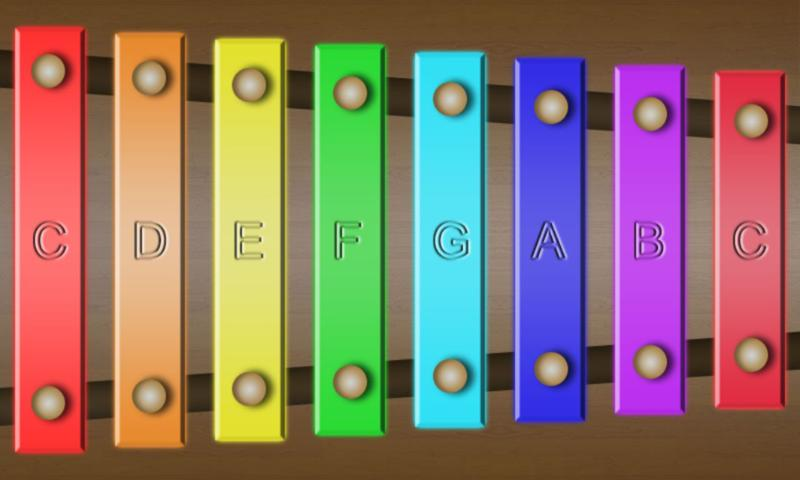
\includegraphics[width=0.36\linewidth]{bar_wrong_ph1.jpeg}
		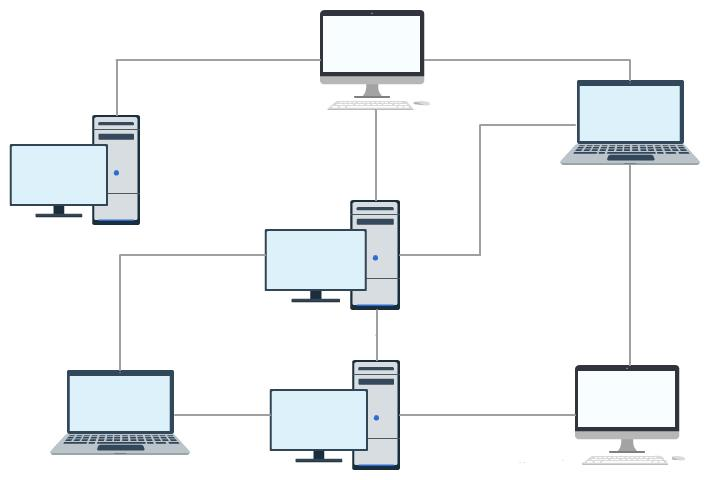
\includegraphics[width=0.36\linewidth]{box_wrong_ph1.jpeg}
		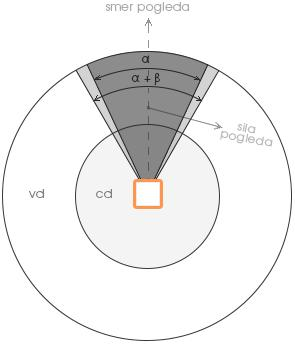
\includegraphics[width=0.24\linewidth]{pie_wrong_ph1.jpeg}
		\caption{\textbf{Images that were wrongly classified as plots.} From left to right we can see images classified as bar plot, box plot and pie chart. None of them is a plot, but if we think in the context of CNNs, we can understand why the model made those mistakes.}
		\label{wrong phase1}
	\end{figure}
	
	In the second phase, when we trained the network again together with those harder examples, it reached 96\% accuracy and a loss of 0.13 on validation data. We will use this model for filtering the extracted images, and will additionally fine tune for different sources, if needed.
	
	%-----------------------------------------------
	\section*{Further work}
	Now we are trying to figure out, what are the attributes, on which we decide whether a plot is good or not. For determining the most popular attributes, we have decided to design some questionnaires and give it to a few people. On those questionnaires will be different plots. For each pair, an individual will decide which one is better and why. For instance \emph{"left plot is better because it has more colors", "right one is better because the axis are labeled",} ... When we will get the results from several questionnaires, we will gather the results and decided what are the most important attributes that make a good plot. From there, we will put our data set of plots on evaluation on Amazon's Mechanical Turk. Workers will be asked similar questions, but now on attributes we have gathered from questionnaires. The plan is to evaluate pairs of pictures, for each which one has better \emph{attribute1, attribute2, ...} After we will have all the data, we are going to build a regression model that will predict how good the plot is and what are the values of its attributes - those should explain why the plot is good/bad.
	
	
	
	% \section*{Results}
	% Pie chart is the best plot.
	
	
	
	%------------------------------------------------
	
	% \section*{Discussion}
	% Do we need this?
	
	
	%------------------------------------------------
	
	% \section*{Acknowledgments}
	% Do we need this?
	
	%----------------------------------------------------------------------------------------
	%	REFERENCE LIST
	%----------------------------------------------------------------------------------------
	\bibliographystyle{unsrt}
	\bibliography{report}
\end{document}